\chapter{Orbital Optimization in Valence Bond Theory}
\label{chap_orbopt}

\ifthenelse{\boolean{wholethesis}}{\relax}{\begin{center}\textit{Generated on \today\ at \currenttime}\end{center}}

\noindent\textbf{Abstract:} The most time consuming step in optimizing a Valence Bond (VB) wave function with VBSCF is the construction of the matrix representation of the Hamilton operator ($\mathbf{H}$) and the corresponding overlap matrix ($\mathbf{S}$) for the wave function and the Brillouin states. In the 1990s a perturbation theory scheme, referred to as approximated Newton-Raphson (aNR), was introduced. For this scheme, less $\mathbf{H}$ matrix elements need to constructed. In this chapter a further approximation is introduced. Instead of calculating $\mathbf{H}$ matrix elements the regular way, they are constructed from Fock matrix elements, taking less time.

\newpage

\section{Introduction}

\lettrine{\initial{I}}{}n 1916 Lewis suggested that atoms share electrons to form chemical bonds \cite{lewis}. Heitler and London incorporated this view a decade later into the quantum chemical description of the covalent bond in H$_2$ \cite{heitler}. In the 1930s Pauling used this description in his famous series of articles on ``The Nature Of The Chemical Bond'' \cite{pauling1,pauling2,pauling3,pauling4,pauling5,pauling6,pauling7,paulingbook}, which earned him the Nobel prize in 1954. This method is nowadays known as the Valence Bond theory.

In Valence Bond theory the wave function is more complex than in many other methods, like the Molecular Orbital theory \cite{hartree1,hartree2,hartree3,fock}. The VB orbitals have no orthogonality restriction and the wave function consists of multiple structures, consisting of one or more Slater determinants. Despite these computational hurdles, Valence Bond theory has kept a decent following through the years \cite{vboverv1,vboverv2,vboverv3}. One of the reasons is the development of powerful computers. On the other hand several efficient methods to optimize Valence Bond wave functions, Spin-Coupled Valence Bond (SCVB) \cite{scvb1,scvb2,scvb3}, Valence Bond Self-Consistent Field (VBSCF) \cite{vbscf1,vbscf2,koos1,zahid} and an algorithm that uses transition density matrices \cite{song}, have been developed.

Like a Valence Bond wave function, a Multi Configurational Self-Consistent Field (MCSCF) \cite{joop,mcscf,roos1,roos2} wave function is expressed in multiple structures, called Configuration State Functions (CSFs), comparable to VB structures. A peculiar difference, though, is the use of orthogonal orbitals in MCSCF. For the optimization of the orbitals in MCSCF, elements from a single Fock matrix, based on the density matrix, can be used \cite{roos1}, because with these elements of the Hamiltonian matrix can be constructed. The Fock matrix has the form:
\begin{equation}
F_{ia} = h_{ia} + \sum_{\sigma\nu} \left\{ \left[ \chi_i \chi_a | \chi_\sigma \chi_\nu \right] - \left[ \chi_i \chi_\nu | \chi_\sigma \chi_a \right] \right\} P^{(\sigma,\nu)},
\label{ch2.eq.fock}
\end{equation}
in which $F_{ia}$ is the Fock matrix element, $\chi_i$ and $\chi_a$ are spin-orbitals, $h_{ia}$ is the one electron integral $\left< \chi_i | \mathbf{h}| \chi_a \right>$. The double sum on the right hand side is over two electron integrals (Coulomb and exchange) times elements of the density matrix $P^{(\sigma,\nu)}$. 

This saves a substantial amount of computation time, because the Fock matrix elements do not depend on the number of determinants in the wave function, while the Hamiltonian matrix elements do. The central question for this chapter is whether it is also possible to use a single Fock matrix for the optimization of the orbitals in VBSCF, although non-orthogonal orbitals are used.

Song \textit{et al.} have shown that a VB wave function can be optimized with the help of transition density matrices from which multiple Fock matrices are constructed \cite{song}. The difference with the approach presented in this chapter is that here only a single Fock matrix is used.
 
At first, the usability of Fock matrix elements in the Hamiltonian matrix is analyzed by comparing the expression for Fock matrix elements, equation \ref{ch2.eq.fock}, with the expression for Hamiltonian matrix elements by L\"{o}wdin \cite{lowdin}:
\begin{equation}
\left< \Delta_p | \hat{H} | \Delta_q \right> = \sum_{ik} h_{ik}S^{(i,k)} + \sum_{i<j,k<l} \left\{ \left[ \chi_i \chi_k | \chi_j \chi_l \right] - \left[ \chi_i \chi_l | \chi_j \chi_k \right] \right\}S^{(i,j,k,l)}  
\label{ch2.eq.lowdindeterminants}
\end{equation}


Following the theoretical section, the implementation of extensions to the perturbation theory (\textit{pert} option) and the new \textit{fock} option in TURTLE will be discussed. After the implementation details, speed-up factors of some test calculations with the \textit{pert} and \textit{fock} options will be presented and compared. Finally, this chapter is concluded with some conclusions and an outlook on future enhancements for the \textit{pert} and \textit{fock} options.  

\section{Theory}

A Valence Bond wave function is constructed from a linear combination of structures:
\begin{equation}
\Psi = \sum_{i} C_i \Phi_i.
\label{ch2.eq.vbwf}
\end{equation}
Such a structure itself is a linear combination of Slater determinants:
\begin{equation}
\Phi = \sum_{i} \alpha_i \Delta_i,
\label{ch2.eq.struct}
\end{equation}
which are antisymmetrized products of spin-orbitals:
\begin{equation}
\Delta = |\chi_i\chi_j\chi_k\chi_l \cdots \chi_n|,
\label{ch2.eq.determ}
\end{equation}
where the spin-orbitals have a spatial part and a spin part which can be $\alpha$ or $\beta$. Two examples are  $\chi_i(\mathbf{x})=\psi_i(\mathbf{r})\alpha(\omega)\equiv\psi_i$ and $\chi_j(\mathbf{x})=\psi_i(\mathbf{r})\beta(\omega)\equiv\overline{\psi_i}$.
Orbitals $\psi$ are linear combinations of one electron basis functions,
\begin{equation}
\psi = \sum_{n} c_n \phi_n,
\label{ch2.eq.basis}
\end{equation}
in which the $c_n$ are orbital coefficients and $\phi_n$ one electron basis functions. The coefficients $C_i$ of the wave function $\Psi$ in equation \ref{ch2.eq.vbwf} and the coefficients $c_n$ of the orbitals $\psi$ in equation \ref{ch2.eq.basis} are variationally determined. 

VBSCF and MCSCF are both based on Super CI \cite{superci1,superci2}, which uses the generalized Brillouin theorem \cite{brillouin,genbrill} as convergence criterium.

A VBSCF wave function is constructed from guess orbitals, which are mostly taken from a Hartree-Fock calculation or are entered manually, \textit{i.e.} the orbitals, which are vectors with coefficients for each basis function, are keyed in by hand. The expectation value of the energy ($E$) for a wave function ($\Psi$) constructed with these orbitals is not necessarily the lowest possible. The expression for the expectation value of the energy is:
\begin{equation}
E = \left < \Psi | \mathbf{H} | \Psi \right >,
\label{ch2.eq.expenerg}
\end{equation}
for a normalized wave function, \textit{i.e.} $\left < \Psi | \Psi \right > = 1$. To lower this value, the orbitals need to be modified, or rather \textit{optimized}. The goal of this optimization is to obtain the orbitals for which $E$ is as low as possible. In that minimum the energy no longer decreases with respect to orbital changes. There are several numerical methods which can be used for finding minima, or roots, of mathematical functions. One of the most popular methods is the Newton-Raphson method \cite{zahid}. A drawback of this method is that its convergence is quadratic. In VBSCF the Super CI approach is used \cite{superci1,superci2}, which, compared to Newton-Raphson, is slightly simpler and has a linear convergence \cite{koos1}. Super CI is explained in the next section.

\subsection{Super CI}

The working of Super CI will be described here in more detail, because the explanations of the approximations in Sections \ref{ch2.sec.anr} and \ref{ch2.sec.fock} are simplified with the definition of the \textit{Brillouin matrix} at hand. In Super CI, the elements in the first column of this Brillouin matrix can be used to check for convergence, as will be made clear hereafter. 

Before modifications in orbitals are discussed, the building blocks of a Valence Bond wave function will be reviewed. Then it will be shown that with clever modifications of the orbitals a minimum in the energy can be found and that then the wave function will fulfill the Brillouin theorem, which states that for optimal orbitals the singly excited Brillouin states do not interact or mix with the ground (or reference) state \cite{brillouin}. 

\subsubsection{Adapting Orbitals}

Orbitals can be changed by adding a portion of an other orbital. For instance, orbital $i$ can be changed by adding a small amount $\delta b_{ia}$ times $a$:
\begin{equation}
i' = i + \delta b_{ia} a.
\label{ch2.eq.orbchange}
\end{equation}
As a simple example, a one determinant wave function $\Psi_0=|i\overline{i}jk|$ with four orbitals is chosen. The orbitals $i$, $j$ and $k$ have $\alpha$ spin, while only $\overline{i}$ has $\beta$ spin. The orbital change of equation \ref{ch2.eq.orbchange} will result in:
\begin{equation}    
\begin{split}
|i'\overline{i'}jk | & = |(i + \delta b_{ia} a)\overline{(i + \delta b_{ia}a)}jk |\\
& = |i\overline{i}jk| + \delta b_{ia}|a\overline{i}jk| + \delta b_{ia} |i\overline{a}jk| + \delta b^2_{ia} |a\overline{a}jk|.\\
\end{split}
\label{ch2.eq.detchange}
\end{equation}
The first term is the original wave function $\Psi_0$. The second and third term are determinants, in which orbital $i$ has been replaced by $a$, once for $\alpha$ and once for $\beta$ spin. In the fourth determinant both occurrences of orbital $i$ have been replaced by $a$. This fourth determinant will be neglected here, because the amount $\delta b_{ia}$ is considered small and hence $\delta b_{ia}^2 \approx 0$.

The combination of the second and third determinant can be created from $|i\overline{i}jk |$ by the single excitation operator $\mathbf{C}_{i \rightarrow a}$, which replaces $i$ by $a$, once for $\alpha$ spin and once for $\beta$ spin \cite{ruttink}. This singly excited structure will be referred to as $\Psi_{ia}$.   The change in $\Psi_0$ caused by the orbital change results (to first order) in:
\begin{equation}
\Psi_{0} \rightarrow \Psi_{0} + \delta b_{ia} \mathbf{C}_{i \rightarrow a} \Psi_{0} = \Psi_{0} + \delta b_{ia} \Psi_{ia}.
\label{ch2.eq.wfchange}
\end{equation}

With this mechanism orbital $i$ could be changed in such a way that the expectation value of the energy of $\Psi_0$ becomes lower. The minimum in the energy is found when the first order derivative of the energy with respect to the orbital change equals zero:
\begin{equation}
\frac{\partial E}{\partial b_{ia}}=\frac{\partial \frac{\left < \Psi_0 | \mathbf{H} | \Psi_0 \right >}{\left < \Psi_0 | \Psi_0 \right >}}{\partial b_{ia}}=0.
\label{ch2.eq.foderiv}
\end{equation}
Making use of the fact that the Hamiltonian and the metric are Hermitian and that the first order derivative with respect to the orbital change of $\Psi_0$ in equation \ref{ch2.eq.wfchange} equals $\Psi_{ia}$ \cite{vbscf2}, the first order derivative of the energy with respect to the orbital change becomes: 
\begin{equation}
\begin{split}
\frac{\partial E}{\partial b_{ia}} & = \frac{2 \cdot \left < \Psi_0 | \mathbf{H} | \Psi_{ia} \right > \left< \Psi_0 | \Psi_0 \right > - 2 \cdot \left < \Psi_0 | \mathbf{H} | \Psi_0  \right > \left< \Psi_0 | \Psi_{ia}\right>}{\left < \Psi_0 | \Psi_0 \right > ^2 }\\
& = \frac{ 2 \cdot \left < \Psi_0 | \mathbf{H} | \Psi_{ia} \right > - 2 \cdot E_0 \left< \Psi_0 | \Psi_{ia} \right >}{\left < \Psi_0 | \Psi_0 \right >}\\
& = \frac{ 2 \cdot \left < \Psi_0 | \mathbf{H} -E_0 | \Psi_{ia} \right >}{\left < \Psi_0 | \Psi_0 \right >}\\
& = 0,
\end{split}
\label{ch2.eq.foderiv2}
\end{equation}
in which $E_0 = \left < \Psi_0 | \mathbf{H} | \Psi_0 \right > / \left < \Psi_0 | \Psi_0 \right >$. Equation \ref{ch2.eq.foderiv2} can be further reduced to:
\begin{equation}
\left < \Psi_0 | \mathbf{H} - E_0 | \Psi_{ia} \right > = 0,
\label{ch2.eq.brillouin}
\end{equation}
which is the Brillouin theorem: with optimal orbitals the singly excited Brillouin state ($\Psi_{ia}$) does not interact or mix with the reference or ground state ($\Psi_0$). 

In equations \ref{ch2.eq.orbchange}-\ref{ch2.eq.brillouin} the effect of a single orbital change has been shown. When all possible excitations from all occupied to all unoccupied orbitals are taken into account, the wave function of equation \ref{ch2.eq.wfchange} becomes:
\begin{equation}
\Psi_{superci} = \Psi_0 + \sum_{ia} b_{ia} \Psi_{ia},
\label{ch2.eq.superci}
\end{equation}
in which $\Psi_{superci}$ is the Super CI wave function, $i$ runs over all occupied orbitals and $a$ runs over all vacant (or virtual) orbitals. Values for $b_{ia}$ can be found by solving the generalized eigenvalue problem:
\begin{equation}
[\mathbf{H}-E_b\mathbf{S}] \cdot \mathbf{b} = 0,
\label{ch2.eq.geig}
\end{equation}
in which $\mathbf{H}$ and $\mathbf{S}$ are the Hamiltonian and metric in the basis of singly excited states ($\Psi_0$ and the $\Psi_{ia}$'s). $E_b$ is the lowest eigenvalue and $\mathbf{b}$ is the corresponding eigenvector. With the elements of $\mathbf{b}$ the orbitals are updated to make $\Psi_0$ equal to $\Psi_{superci}$ to first order:
\begin{equation}
i' = i + \sum_{a} b_{ia} a.
\label{ch2.eq.orbupd}
\end{equation}
With the modification of the orbitals the Super CI wave function is contracted or condensed into $\Psi_0$. This is exemplified for the change in orbital $i$ in the simple one determinant wave function in equation \ref{ch2.eq.detchange}. Orbital $i$ in $\Psi_0$ is modified with $\delta b_{ia}$ times orbital $a$, which results in determinant $|i'\overline{i'}jk |$:
\begin{equation}
\begin{split}
\Psi_{0} \leftarrow & \Psi_{0} + \delta b_{ia} \Psi_{ia} = \\
&|i\overline{i}jk| + \delta b_{ia}(|a\overline{i}jk| + |i\overline{a}jk|) = \\
&|(i + \delta b_{ia}a)\overline{(i + \delta b_{ia}a)}jk| = \\
&|i'\overline{i'}jk |.\\
\end{split}
\label{ch2.eq.condense}
\end{equation}
So, $\Psi_0$ will contain the updated orbital $i'$ which will be denoted $i$ in the next step (iteration). This procedure for a single orbital update is performed for all combinations in the summation in the Super CI wave function. Since the orbital changes are performed independently, they may be counteracting and therefore the Brillouin condition may not be fulfilled in a single step. Therefore, a new excitation pattern for a new $\Psi_{superci}$ is created. The eigenvalue problem is solved again and the orbitals are updated once more. It is expected that the orbital updates become smaller with each step. This procedure is repeated until all Brillouin elements, $\left < \Psi_0 | \mathbf{H} - E_0 | \Psi_{ia} \right >$, have become zero. At that point the expectation value of the energy ($E_0$) is stationary with respect to orbital changes (equation \ref{ch2.eq.foderiv2}).

Up till here, $\Psi_0$ was constructed of a single determinant, \textit{i.e.} $|i\overline{i}jk|$. A regular VB wave function consists of multiple structures, and hence multiple determinants (see equations \ref{ch2.eq.vbwf} and \ref{ch2.eq.struct}). In that case, the contraction of equation \ref{ch2.eq.condense} will contain more determinants, all in which orbital $i$ has been replaced by $a$. With the expansion of the wave function into multiple structures/determinants, there are two points to consider. Firstly, besides the occupied and virtual orbital classes, a third class occurs: one with partly occupied orbitals. This class comprises orbitals which occur in some determinants, but not in all. Secondly, after each orbital optimization step, the structure coefficients $C_i$ (equation \ref{ch2.eq.vbwf}) should be recalculated with the newly optimized orbitals. With these new structure coefficients, a new orbital optimization procedure should be performed. Ultimately, convergence is reached when both orbitals \textit{and} structure coefficients no longer change.

An example of a Brillouin matrix, which contains elements resulting from two excitations: an excitation from $i$ to $a$ ($\Psi_{ia}$) and one from $i$ to $b$ ($\Psi_{ib}$), is shown below\footnote{Note that only the lower triangle of this Hermitian matrix is shown.}:
\begin{equation}
\left[\begin{array}{ccc}
\left< \Psi_{0} | \mathbf{H}-E_0 | \Psi_{0} \right> & & \\
\left< \Psi_{0} | \mathbf{H}-E_0 | \Psi_{ia} \right> & \left< \Psi_{ia} | \mathbf{H}-E_0 | \Psi_{ia} \right> &\\
\left< \Psi_{0} | \mathbf{H}-E_0 | \Psi_{ib} \right> & \left< \Psi_{ia} | \mathbf{H}-E_0 | \Psi_{ib} \right> & \left< \Psi_{ib} | \mathbf{H}-E_0 | \Psi_{ib} \right> \\
\end{array}\right].
\label{ch2.eq.hamilt}
\end{equation}
The Brillouin matrix is the $\mathbf{H}$ matrix minus $E_0$ \cite{koos1} and hence has the same dimension as the $\mathbf{H}$ and $\mathbf{S}$ matrices in equation \ref{ch2.eq.geig}. For each extra excitation the $\mathbf{H}$, $\mathbf{S}$ and Brillouin matrices are extended with one extra row and column. Hence, the number of elements increases roughly quadratic with the number of excitations. A nice side effect of constructing the Brillouin matrix with $E_0$ present is that with it, it is rather easy to check for convergence: the elements in the first column are zero when convergence is reached.

The calculation of the elements in $\mathbf{H}$ is expensive because of the large number of determinants, caused by the expansion into the Super CI wave function: for each excitation a Brillouin state, containing 1 to 2 times the number of determinants of $\Psi_0$, is added. For each determinant combination the evaluation of (large amounts of) subdeterminants \cite{koos2}, or cofactors\footnote{Cofactors are described in detail in Appendix A.} are required. Considering this, van Lenthe \textit{et al.} asked themselves whether all the elements in the $\mathbf{H}$ matrix, like $\left < \Psi_{ia} | \mathbf{H} - E_0 | \Psi_{ib} \right >$ for example, would be required for convergence to the Brillouin condition, or that less elements would suffice \cite{koos1}. They presented a new method, referred to as approximated Newton-Raphson (Section \ref{ch2.sec.anr}), which requires less $\mathbf{H}$ and $\mathbf{S}$ matrix elements than regular Super CI.

Another question, which will be discussed after the description of approximated New{-}ton-Raphson method, is whether it would be possible to calculate certain $\mathbf{H}$ matrix elements, \textit{i.e.} the first column element and the diagonal element, in a cheaper or faster way. 

\subsection{\label{ch2.sec.anr}The Approximated Newton-Raphson Method}

In the approximated Newton-Raphson technique perturbation theory is used to obtain orbital update coefficients. These coefficients are approximated by the quotient of the first column element and the diagonal element on each row of equation \ref{ch2.eq.hamilt}:
\begin{equation}
b_{ia}= - \frac{\left< \Psi_{0} | \mathbf{H}-E_0 | \Psi_{ia} \right>}{\left< \Psi_{ia} | \mathbf{H}-E_0 | \Psi_{ia} \right>}.
\label{ch2.eq.anr}
\end{equation}
This means that elements of the type $\left< \Psi_{ia} | \mathbf{H}-E_0 | \Psi_{ib} \right>$ are not used. In that way, only two matrix elements need to be calculated for such an excitation, instead of $m$, where $m$ equals the total number of excitations. This reduces the quadratic increase in number of matrix elements to linear.

When the orbitals are optimal the numerator in equation \ref{ch2.eq.anr} becomes zero (Brillouin condition). In that case the orbital updates ($b_{ia}$) become zero and the orbitals no longer change. It is stressed that the approximation in aNR is in the calculation of the update coefficients, rather than in the total energy $E$. Therefore the total energy for an aNR calculation should not differ from a regular Super CI calculation.

A further reduction of the calculation time can be achieved, when both the numerator and the denominator in equation \ref{ch2.eq.anr} could be calculated faster, given that the number of iterations does not explode. The numerator, though, can not be approximated, since it is used as convergence criterion (equation \ref{ch2.eq.brillouin}). So the ``faster'' method must result in exactly the same value as for the regular Brillouin matrix element. The denominator in equation \ref{ch2.eq.anr} is used as a weighting factor and therefore it may be approximated. Rough approximations, however, may lead to very slow convergence, or even divergence. 

Using a Fock matrix the numerator may be calculated faster in some cases. In the next section the applicability of Fock matrix elements will be analyzed: in which situations are they equal to the elements in the first column of the Brillouin matrix and can they be used?

\subsection{\label{ch2.sec.fock}Fock Matrix Elements} 

A Multi Configuration Self-Consistent Field (MCSCF) \cite{wahldasbook,daswahl} wave function is expressed in Configuration State Functions (CSF's). This structure is comparable with the expression of a VB wave function in structures: the CSF's are comparable to VB structures in the sense that both are constructed from fixed combinations of determinants. Two major differences are that both bonding \textit{and} anti-bonding orbitals occur in CSF's and that the molecular orbitals are chosen orthogonal in MCSCF. A special case of an MCSCF wave function is the Complete Active Space Self-Consistent Field (CASSCF) wave function. A CASSCF wave function contains all distinctive configurations that can be created from the total number of electrons in all molecular orbitals, while in MCSCF only a subset of these configurations is used. Here, the terms MCSCF and CASSCF are intermixed, because only the general form of this type of wave function is important. The similarity in structure justifies a closer look at the orbital optimization techniques in MCSCF, which might also be applicable to VBSCF.

For the optimization of doubly occupied orbitals in MCSCF wave functions Fock matrix elements can be used, since those are, except for a constant factor, equal to Brillouin matrix elements of the type $\left < \Psi_0 | \mathbf{H} | \Psi_{ia} \right >$ \cite{roos1,roos2}:
\begin{equation}
%roos1 - equation 23a - page 163
\left < \Psi_0 | \mathbf{H} | \Psi_{ia} \right > = 2^{\frac{1}{2}}F_{ia},
\label{ch2.eq.mcscffock}
\end{equation}
in which $F_{ia}$ is equal to $\left < i | \mathbf{f} | a \right > $, which is an element of a Fock matrix on MO basis. Such a Fock matrix element is calculated by transforming the Fock matrix on AO basis, constructed from the one and two electron integrals and the one electron density matrix, to MO basis. This means that for this transformation the number of structures and determinants, \textit{i.e.} the complexity of the wave function, is irrelevant because they are not needed. The possible application of this method could lead to a decrease in calculation time for VBSCF as well. Besides, the fact that the Fock matrix element is \textit{equal} to the Brillouin matrix element, at least in MCSCF, makes it in principle applicable as numerator in equation \ref{ch2.eq.anr}.  

\subsubsection{Doubly Occupied Orthogonal Orbitals}

For the analysis of the applicability of Fock matrix elements, a VBSCF wave function with orthogonal doubly occupied orbitals, which occur in every structure, is chosen. In analogy with MCSCF, any structure ($\Phi_i$) in a VB wave function can be written as:
\begin{equation}
%thor4 - equation 2 - page 69
\Phi_i = \mathcal{A}(\Phi^{\mathrm{core}} \times \Phi_i^{\mathrm{active}}),
\label{ch2.eq.wfsplit}
\end{equation}
in which $\mathcal{A}$ is the antisymmetrizer, $\Phi^{\mathrm{core}}$ is the product of all doubly occupied orbitals, which is equal for all structures, and $\Phi_i^{\mathrm{active}}$ is the product of the active (or variably) occupied orbitals in structure $\Phi_i$. Although not necessary, it is convenient to orthogonalize as many orbitals onto each other as possible \cite{vbscf2}. This results in the two occupied orbital subsets mentioned here, the core, or always doubly occupied orbitals and the active orbitals. The remaining unoccupied, or virtual orbitals are mostly chosen orthogonal to all other orbitals. For a detailed description of the construction of the virtual subspace, see the first appendix in reference \cite{koos1}.

In the active subspace, the orbitals are not necessarily orthogonal to each other. In principle, however, these orbitals could be transformed in such a way that they become orthogonal to each other. In practice, such transformations are performed by Thorsteinsson \textit{et al.} in their Complete Active Space Valence Bond (CASVB) method \cite{thor1,thor2,thor3,thor4}. In the CASVB method a CASSCF wave function is taken for a start. By orbital transformations, which need not be unitary, an alternative representations of exactly the same wave function is obtained, based instead on non-orthogonal orbitals, such as those that are more characteristic of VB. The initial main motivation behind CASVB was to be able to use modern VB language, whilst avoiding the need to carry out actual VB calculations, which were traditionally perceived to be somewhat more expensive. Here, the transformation will be used in the opposite direction: from a VB wave function to a CASSCF wave function. With such a transformation the wave function becomes:
\begin{equation}
%thor4 - equation 1 - page 68
\Psi_0 = \sum_{i}^{n} C_i \Phi_i = \sum_{j}^{m} D_j \Phi^{\mathrm{\bot }}_j,
\label{ch2.eq.vbtrans}
\end{equation}
in which the $\Phi^{\mathrm{\bot }}_j$'s are structures containing orthogonal orbitals and the $D_j$'s are the corresponding structure coefficients. With this transformation a CASSCF wave function with orthogonal orbitals is created without changing neither the expectation value of the energy, nor the one electron density matrix (and hence the Fock matrix) on AO basis. Because the orbitals in the core and virtual subspace are already orthogonal, members of these subspaces can be kept constant during the transformation. This means that the Fock matrix elements of the type $F_{ia}$ remain unmodified, because the one and two electron integrals and the one electron density matrix on AO basis \textit{and} the orbitals $i$ and $a$ remain the same.

So, without performing any transformation $F_{ia}$-type Fock matrix elements can be used in VBSCF for the optimization of doubly occupied \textit{orthogonal} orbitals, because the rules derived for MCSCF can be applied. This means that instead of calculating Brillouin matrix elements of the type $\left < \Psi_0 | \mathbf{H} | \Psi_{ia} \right >$, Fock matrix elements of the type $\left < i | \mathbf{f} | a \right > $ taken from Fock matrix on MO basis, can be used (equation \ref{ch2.eq.mcscffock}).

Up till here, the doubly occupied orbitals in the VB wave function were chosen (or made) orthogonal to each other. This is not always possible, or even desirable. Quite often a VB wave function is constructed to investigate the bonding between two molecular fragments. In that case doubly occupied orbitals on one fragment are generally not orthogonal to the orbitals on the other fragment, because they are only expressed in a local subset of AO's, \textit{i.e.} those on its own fragment. This method, with orbitals on fragments, is denoted as \textit{local} VBSCF, while the method in which the orbitals are allowed to spread over the whole molecule is referred to as \textit{delocal} VBSCF.

\subsubsection{Non-Orthogonal Orbitals}

To analyze the impact of the non-orthogonal orbitals in a VB wave function on the applicability of a Fock operator a simple single determinant wave function $\Psi_0 = N |ijkl \cdots n|$, in which $N$ is the normalization coefficient,  is selected. With the $\mathbf{C}_{i \rightarrow a}$ operator $\Psi_{ia} = N |ajkl \cdots n|$,  the singly excited determinant, is generated.

In this chapter overlaps between Slater determinants, like those in $\Psi_0$ and $\Psi_{ia}$, are written in terms of cofactors, which are determinants of orbital overlaps. The overlap of wave function $\Psi_0$ with $\Psi_{ia}$ can be expressed in the cofactor $S_{0(i\rightarrow a)}^{(0)}$ (equation \ref{ch2.eq.s0ia}). The superscript $(0)$ indicates that this is a zeroth order cofactor. The subscript $0(i\rightarrow a)$ indicates that this determinant contains overlaps of orbitals in $\Psi_0$ $(0)$ with the orbitals of $\Psi_{ia}$ ($(i\rightarrow a)$). In the cofactor the rows and columns are labeled: the columns are labeled with the orbitals of $\Psi_0$ and the rows with the orbitals of $\Psi_{ia}$: 
\begin{equation}
\left < \Psi_0 | \Psi_{ia} \right> = N^2 \cdot S_{0(i\rightarrow a)}^{(0)} = N^2 \cdot
\begin{array}{lllllll}
 &  i & j & k & l & \cdots & n \\
 a &  \multicolumn{1}{|l}{ s_{ia} } & s_{ja} & s_{ka} & s_{la} & & \multicolumn{1}{l|}{ s_{na} } \\
 j & \multicolumn{1}{|l}{ s_{ij} } & 1 & s_{kj} & s_{lj} & & \multicolumn{1}{l|}{s_{nj}} \\
 k & \multicolumn{1}{|l}{ s_{ik} } & s_{jk} & 1 & s_{lk} & & \multicolumn{1}{l|}{s_{nk}} \\
 l & \multicolumn{1}{|l}{ s_{il} } & s_{jl} & s_{kl} & 1 & & \multicolumn{1}{l|}{s_{nl}} \\
 \vdots & \multicolumn{1}{|l}{ } &   &   & & \ddots & \multicolumn{1}{l|}{\vdots} \\
 n & \multicolumn{1}{|l}{ s_{in} } & s_{jn} & s_{kn} & s_{ln} & \cdots & \multicolumn{1}{l|}{1}
\end{array}.
\label{ch2.eq.s0ia}
\end{equation}
In the cofactor above the element $s_{ij}$, for example, is the overlap between orbital $i$ and $j$.

The Brillouin matrix element for the two determinants in $\Psi_0$ and $\Psi_{ia}$ can be expressed in three parts, using L\"{o}wdin's formula \cite{lowdin}, in which first order cofactors have a superscript with two indices, while second order cofactors have four indices in their superscripts:
\begin{equation}
\begin{split}
\left < \Psi_0 | \mathbf{H} - E_0 | \Psi_{ia} \right>= & + N^2 \sum_{\rho\tau} h_{\rho\tau} S_{0(i\rightarrow a)}^{(\rho,\tau)} \\
& + N^2 \sum_{\rho<\sigma,\tau<\nu} [\left <\rho\sigma|\tau\nu \right > - \left < \rho\sigma | \nu\tau \right> ]  S_{0(i\rightarrow a)}^{(\rho,\sigma,\tau,\nu)} \\
&  - E_0 N^2 S_{0(i\rightarrow a)}^{(0)}.\\
\end{split}
\label{ch2.eq.lowdin}
\end{equation}
In this formula the summation indices $\rho$, $\sigma$, $\tau$ and $\nu$ run over all orbitals in the determinants of $\Psi_0$ and $\Psi_{ia}$. Firstly, there is a series of one electron integrals $h_{\rho\tau}$ multiplied by first order cofactors $S_{0(i\rightarrow a)}^{(\rho,\tau)}$. One of these cofactors is $S_{0(i\rightarrow a)}^{(i,a)}$:
\begin{equation}
S_{0(i\rightarrow a)}^{(i,a)} =
\begin{array}{lllllll}
 &  \hskip 2.0 pt \hbox{\lower 120pt\hbox{\vrule height128pt width 1.0pt}}\hskip-3.0pt i & j & k & l & \cdots & n \\
\noalign{\vskip-115pt}
 a &  \multicolumn{1}{|l}{s_{ia}} & s_{ja}  & s_{ka} & s_{la} & & \multicolumn{1}{l|}{ s_{na} } \\
\noalign{\vskip-8pt}
\multispan7\hbox{\vrule  height 1.0 pt width164pt}\cr
\noalign{\vskip 7pt}
  j & \multicolumn{1}{|l}{s_{ij}} & 1 & s_{kj} & s_{lj} & & \multicolumn{1}{l|}{s_{nj}} \\
 k & \multicolumn{1}{|l}{s_{ik}} & s_{jk} & 1 & s_{lk} & & \multicolumn{1}{l|}{s_{nk}} \\
 l & \multicolumn{1}{|l}{s_{il}} & s_{jl} & s_{kl} & 1 & & \multicolumn{1}{l|}{s_{nl}} \\
 \vdots & \multicolumn{1}{|l}{ } &   &   & & \ddots & \multicolumn{1}{l|}{\vdots} \\
 n & \multicolumn{1}{|l}{ s_{in}} & s_{jn} & s_{kn} & s_{ln} & \cdots & \multicolumn{1}{l|}{1}
\end{array}.\\
\label{ch2.eq.examfoco}
\end{equation}
Compared to the zeroth order cofactor in equation \ref{ch2.eq.s0ia}, the dimension of this determinant is one row and column smaller. 

The second part in equation \ref{ch2.eq.lowdin} consists of Coulomb and exchange integrals, $\left <\rho\sigma|\tau\nu \right >$ and $\left < \rho\sigma | \nu\tau \right>$ respectively, multiplied by second order cofactors $S_{0(i\rightarrow a)}^{(\rho,\sigma,\tau,\nu)}$. An example of such a second order cofactor is:
\begin{equation}
S_{0(i\rightarrow a)}^{(i,k,a,l)} =
\begin{array}{lllllll}
 &  \hskip 2.0 pt \hbox{\lower 120pt\hbox{\vrule height128pt width 1.0pt}}\hskip-3.0pt i & j & \hskip 2.0 pt \hbox{\lower 120pt\hbox{\vrule height128pt width 1.0pt}}\hskip-3.0pt k & l & \cdots & n \\
\noalign{\vskip-115pt}
 a &  \multicolumn{1}{|l}{s_{ia}} & s_{ja}  & s_{ka} & s_{la} & & \multicolumn{1}{l|}{ s_{na} } \\
 \noalign{\vskip-8pt}
\multispan7\hbox{\vrule  height 1.0 pt width164pt}\cr
\noalign{\vskip 7pt}
 j & \multicolumn{1}{|l}{s_{ij}} & 1 & s_{kj} & s_{lj} & & \multicolumn{1}{l|}{s_{nj}} \\
 k & \multicolumn{1}{|l}{s_{ik}} & s_{jk} & 1 & s_{lk} & & \multicolumn{1}{l|}{s_{nk}} \\
 l & \multicolumn{1}{|l}{s_{il}} & s_{jl} & s_{kl} & 1 & & \multicolumn{1}{l|}{s_{nl}} \\
 \noalign{\vskip-8pt}
\multispan7\hbox{\vrule  height 1.0 pt width164pt}\cr
\noalign{\vskip 7pt}
 \vdots & \multicolumn{1}{|l}{ } &   &   & & \ddots & \multicolumn{1}{l|}{\vdots} \\
 n & \multicolumn{1}{|l}{ s_{in}} & s_{jn} & s_{kn} & s_{ln} & \cdots & \multicolumn{1}{l|}{1}
\end{array}.\\
\label{ch2.eq.examsoco}
\end{equation}
Compared to the first order cofactor in equation \ref{ch2.eq.examfoco}, this determinant has one row and column less. For more information on cofactors, the reader is referred to Appendix A. 

The last part in equation \ref{ch2.eq.lowdin} is the ground state energy $E_0$ multiplied by the zeroth order cofactor $S_{0(i\rightarrow a)}^{(0)}$, which has already been shown in equation \ref{ch2.eq.s0ia}.

Compared with the complexity of the expression of a matrix element in L\"{o}wdin's formula (equation \ref{ch2.eq.lowdin}), the expression for a Fock matrix element as used for the optimization of doubly occupied orbitals in MCSCF, is relatively simple \cite{roos1}:
\begin{equation}
F_{ia} = h_{ia} + \sum_{\sigma \nu} [ \left <i \sigma | a \nu \right > - \left < i \sigma | \nu a \right> ]P^{(\sigma,\nu)},
\label{ch2.eq.fockgen}
\end{equation}
in which $h_{ia}$ is a one electron integral of the type $\left < i | \mathbf{h} | a \right> $ followed by the sum over orbital indices $\sigma$ and $\nu$ of differences between Coulomb and exchange integrals, multiplied by elements of a first order density matrix $P^{(\sigma,\nu)}$. To analyze whether Fock matrix elements are equal to Brillouin matrix elements in VBSCF, the constituents, \textit{i.e.} the one and two electron integrals and the density matrix, are taken from VB and used in equation \ref{ch2.eq.fockgen}, in anology with MCSCF. The elements of a VB density matrix can be expressed in first order cofactors \cite{joopboek}:
\begin{equation}
P^{(\sigma,\nu)} = \sum_{pq}  C_p C_q S_{pq}^{(\sigma,\nu)},
\label{ch2.eq.densmat1}
\end{equation}
in which $C_p$ and $C_q$ are determinant coefficients that are multiplied with the first order cofactor belonging to the determinant combination $p$ with $q$.  The summation indicates that the total one electron density matrix is constructed from contributions of determinant combinations. For the single determinant wave function $\Psi_0 = N |ijkl \cdots n|$, which is being examined here, this then reduces to a single cofactor:
\begin{equation}
P^{(\sigma,\nu)} = N^2 S_{00}^{(\sigma,\nu)}.
\label{ch2.eq.densmat2}
\end{equation}
  
For $\left < \Psi_0 | \mathbf{H} - E_0 | \Psi_{ia} \right >$ to be equal to $F_{ia}$ the separate parts, \textit{i.e.} the one electron integral part, the two electron integral part and the $E_0$ part, have to be equal, which leads to the following set of equations\footnote{The "$\stackrel{?}{=}$" symbol means that the conditions for equality will be investigated.}:
\begin{equation}
h_{ia} \stackrel {?}{=} N^2 \sum_{\rho\tau} h_{\rho\tau} S_{0(i\rightarrow a)}^{(\rho,\tau)},
\label{ch2.eq.oneelpart}
\end{equation}
\begin{equation}
\sum_{\sigma \nu} [ \left <i \sigma | a \nu \right > - \left < i \sigma | \nu a \right> ]S_{00}^{(\sigma,\nu)} \stackrel {?}{=}  \sum_{\rho<\sigma,\tau<\nu} [\left <\rho\sigma|\tau\nu \right > - \left < \rho\sigma | \nu\tau \right> ]  S_{0(i\rightarrow a)}^{(\rho,\sigma,\tau,\nu)},
\label{ch2.eq.twoelpart}
\end{equation}
\begin{equation}
0 \stackrel {?}{=} E_0 N^2 S_{0(i\rightarrow a)}^{(0)}.
\label{ch2.eq.e0part}
\end{equation}

The difference between the one electron integral part of the Fock matrix element and the Brillouin matrix element is that the Fock matrix element only contains a single one electron integral, while the Brillouin matrix element contains a whole series. This series can be split up in four terms, of which the first is $h_{ia}$ multiplied with the first order cofactor $S_{0(i\rightarrow a)}^{(i,a)}$: 
\begin{equation}
\begin{split}
h_{ia} &\stackrel {?}{=} N^2 \sum_{\rho\tau} h_{\rho\tau} S_{0(i\rightarrow a)}^{(\rho,\tau)}\\
&\stackrel {?}{=} N^2 (h_{ia} S_{0(i\rightarrow a)}^{(i,a)} + \sum_{\rho \ne i} h_{\rho a} S_{0(i\rightarrow a)}^{(\rho,a)} +  \sum_{\tau \ne a} h_{i\tau} S_{0(i\rightarrow a)}^{(i,\tau)} + \sum_{\rho \ne i, \tau \ne a} h_{\rho\tau} S_{0(i\rightarrow a)}^{(\rho,\tau)}).
\end{split}
\label{ch2.eq.oneelpart2}
\end{equation}

The last three summations on the right hand side, \textit{viz} the first order cofactors in which the combination of orbital $i$ and $a$ has not been removed, are not present in the Fock matrix element and should therefore vanish in the Brillouin matrix element. An example from the second term of a one electron integral contribution to the Brillouin matrix element and not to the Fock matrix element is $h_{ja} \cdot S_{0(i\rightarrow a)}^{(j,a)}$:
\begin{equation}
h_{ja}\cdot S_{0(i\rightarrow a)}^{(j,a)} = h_{ja} \cdot
\begin{array}{lllllll}
 & i & \hskip 2.0 pt \hbox{\lower 120pt\hbox{\vrule height128pt width 1.0pt}}\hskip-3.0 pt j & k & l & \cdots & n \\
\noalign{\vskip-115pt}
 a &  \multicolumn{1}{|l}{ s_{ia} } & s_{ja} & s_{ka} & s_{la} & & \multicolumn{1}{l|}{ s_{na} } \\
\noalign{\vskip-8pt}
\multispan7\hbox{\vrule  height 1.0 pt width164pt}\cr
\noalign{\vskip 7pt}
 j & \multicolumn{1}{|l}{ s_{ij}} & 1 & s_{kj} & s_{lj} & & \multicolumn{1}{l|}{s_{nj}} \\
 k & \multicolumn{1}{|l}{ s_{ik}} & s_{jk} & 1 & s_{lk} & & \multicolumn{1}{l|}{s_{nk}} \\
 l & \multicolumn{1}{|l}{ s_{il}} & s_{jl} & s_{kl} & 1 & & \multicolumn{1}{l|}{s_{nl}} \\
 \vdots & \multicolumn{1}{|l}{ } &   &   & & \ddots & \multicolumn{1}{l|}{\vdots} \\
 n & \multicolumn{1}{|l}{ s_{in}} & s_{jn} & s_{kn} & s_{ln} & \cdots & \multicolumn{1}{l|}{1}
\end{array}.\\
\label{ch2.eq.case2}
\end{equation}
This contribution can only vanish when the cofactor is zero, which means that a row or a column needs to be zero. This cofactor is zero only when the elements in the first column ($s_{ij}$, $s_{ik}$, $s_{il} ... s_{in}$) are zero; other columns contain a "1" on the diagonal positions and therefore not all elements can be ``nilled''. This also guarantees that other cofactors in this second term are then also zero, which can be seen by moving the vertical line through column $j$ to column $k$, $l \cdots n$. 

In analogy, the cofactors in the third term ($S_{0(i\rightarrow a)}^{(i,\tau)}$) are only zero when the elements in the first row ($s_{ja}$, $s_{ka}$, $s_{la} \cdots s_{na}$) are zero (moving the horizontal line from row $j \cdots n$ with the vertical line through column $i$). 

Finally, the cofactors in the fourth term only become zero when $s_{ia}$ is also zero (horizontal and vertical lines through rows and columns from $j \cdots n$ in equation \ref{ch2.eq.case2}). 

The restriction that the elements in the first row and column of $S_{0(i\rightarrow a)}^{(j,a)}$ ($s_{ia}$, $s_{ij}$, $s_{ik}$, $s_{il}$, $s_{in}$, $s_{ja}$, $s_{ka}$, $s_{la}$ and $s_{na}$) need to be zero indicates that orbital $i$ and $a$ must be chosen orthogonal to each other and to all other orbitals, which rules out the use of Fock matrix elements as aids for the optimization of non-orthogonal orbitals. 

Furthermore, there is no restriction for the orthogonality amongst virtual orbitals, because the Brillouin matrix elements in the first column, except $\left< \Psi_0 | \mathbf{H} - E_0 | \Psi_0 \right>$, only contain a singly excited structure, \textit{viz.} $\Psi_{ia}$. Therefore, only one virtual orbital will be present in \textit{all} determinants.

Because of the orthogonality restrictions which follow from the analysis of equation \ref{ch2.eq.oneelpart}, the other comparisons in equations \ref{ch2.eq.twoelpart} and \ref{ch2.eq.e0part} will not be discussed here, because with orthogonal orbitals $i$ and $a$ the situation explained in Section \ref{ch2.sec.fock} - \textbf{Doubly Occupied Orthogonal Orbitals} is obtained.

\subsubsection{\label{ch2.sec.denominator}Approximation Of The Denominator}

As stated before, the numerator in equation \ref{ch2.eq.anr} is needed to check whether the minimum in the energy is reached and therefore the Fock matrix element has got to be equal to the Brillouin matrix element. For the denominator, there is no such hard condition, since it is only used as weighting factor. 

The diagonal element in the Brillouin matrix is:
\begin{equation}
\left< \Psi_{ia} | \mathbf{H}-E_0 | \Psi_{ia} \right>  =  \left< \Psi_{ia} | \mathbf{H} | \Psi_{ia} \right>  - E_0 \left< \Psi_{ia} | \Psi_{ia} \right>.
\label{ch2.eq.brildiag}
\end{equation}
The difference between $\left < \Psi_{ia} | \mathbf{H} | \Psi_{ia} \right >$ and $E_0 \left< \Psi_{ia} | \Psi_{ia} \right>$ can be approximated with the help of Fock matrix elements on the diagonal:
the expectation value of the energy of the excited state ($\left< \Psi_{ia} | \mathbf{H} | \Psi_{ia} \right>$) is roughly the ground state energy ($E_0$, $\Psi_{ia}$ is not normalized: part of the approximation) minus the energy of the no longer occupied orbital $i$ (roughly $F_{ii}$) plus the energy of the newly occupied $a$ (roughly $F_{aa}$). The denominator then becomes:
\begin{equation}
\frac{\left< \Psi_{ia} | \mathbf{H}-E_0 | \Psi_{ia} \right>}{\left< \Psi_{ia} | \Psi_{ia} \right>} \approx (F_{aa}-F_{ii}).
\label{ch2.eq.cheapdiag}
\end{equation}
This is an approximation, since removing an orbital will influence other orbitals, which is not taken into account here. This approximation may or may not work. An advantage of approximating the diagonal Brillouin matrix element with the difference of two Fock matrix elements is that it saves time, especially when the wave function consists of a lot of determinants. On the other hand, since it is an approximation it might result in more iterations. This means that in some situations/calculations it will speed up, while in others it won't.

\section{\label{ch2.sec.implementation}Implementation}

The implementation of the approximations described in the previous section consists of two parts. Firstly, the approximated Newton-Raphson method, which was already implemented in TURTLE, has been extended with extra options. Secondly, the use of a Fock matrix for the optimization of doubly occupied orbitals has been implemented from scratch.

In the original aNR implementation the perturbation (equation \ref{ch2.eq.anr}) was used for excitations from the always and partly occupied orbitals to the virtuals. For all other excitations, \textit{i.e.} those from the always occupied orbitals to the partly occupied orbitals and from partly occupied to other partly occupied orbitals, an $\mathbf{H}$ and $\mathbf{S}$ matrix were constructed, for which the update coefficients were retrieved by solving the generalized eigenvalue problem (equation \ref{ch2.eq.geig}). 

In the current implementation there are three optimization options per excitation. The first option is that the excitation is treated with Super CI. In that case all interaction elements will be calculated. These are the interaction element of the ground state with the singly excited state, like $\left < \Psi_{0} | \mathbf{H} - E_0 | \Psi_{ia} \right >$, the diagonal element, $\left < \Psi_{ia} | \mathbf{H} - E_0 | \Psi_{ia} \right >$, and all interaction elements with other singly excited structures, like $\left < \Psi_{ia} | \mathbf{H} - E_0 | \Psi_{ib} \right >$. Please note, that these latter elements are only calculated when both excitations ($i \rightarrow a$ and $i \rightarrow b$) are treated with Super CI.

The second option is that the excitation is treated with approximated Newton-Raphson. In that case only the two matrix elements in equation \ref{ch2.eq.anr} are calculated to obtain the update coefficient $b_{ia}$.

In the third option the excitation is treated with the Fock operator. In that case the orbital update coefficient $b_{ia}$ is calculated by dividing the Fock matrix element of the type $F_{ia}$ by the difference between $F_{ii}$ and $F_{aa}$ (Section \ref{ch2.sec.denominator}):
\begin{equation}
b_{ia}= - \frac{F_{ia}}{F_{aa}-F_{ii}}.
\label{ch2.eq.fockapprox}
\end{equation}

For excitations treated with regular Super CI, the $\mathbf{b}$ vector is calculated by solving the generalized eigenvalue problem (equation \ref{ch2.eq.geig}). This eigenvector is then padded with the separately calculated update coefficients of equations \ref{ch2.eq.anr} and \ref{ch2.eq.fockapprox}. With the elements from of this $\mathbf{b}$ vector the orbitals are updated, like in equation \ref{ch2.eq.condense}.

The three options above suggest that the user needs to specify beforehand which Brillouin matrix rows (or excitations) should be treated with which option. Since the virtual space is not yet created at the beginning of the calculation it is not very practical to specify the optimization method per excitation. Therefore, two additional specification options have been added: the specification per occupied orbital and the specification per orbital class. All excitations for either a certain orbital or all orbitals in a class are treated with the same option, be-it \textit{superci}, \textit{pert} or \textit{fock}. There are three orbital classes: doubly occupied (doc), variably occupied (voc) and unoccupied (uoc). The doubly occupied class contains orbitals that occur twice in each determinant, once with $\alpha$ and once with $\beta$ spin. The variably occupied class contains orbitals which occur in some determinants and the unoccupied orbital class contains orbitals which only occur in excited state structures. It should be noted that the \textit{fock} option can only be used for the optimization of orbitals which are orthogonal to all other orbitals. The most commonly used specification option, at least for the calculations reported in this thesis, is the specification per orbital class. 

\section{Sample Calculations}

In this section results from a few test calculations will be presented. In the first example some of the new parameters for the extended \textit{pert} option are tested. The results are compared to those from a complete Super CI calculation. In the second example results from several calculations with the \textit{superci}, the \textit{pert} and the new \textit{fock} option are compared.  

\subsection{\label{ch2.sec.cyclopent}First Example: The Cp-SiH Molecule}

For the work described in Chapter \chcyclopentadienyl\ a number of local VBSCF calculations have been performed to investigate the bonding mechanism of main group metal hydrides to cyclopentadienyl moieties. For details on the geometry optimization and the basis sets used, see Chapter \chcyclopentadienyl\ and reference \cite{budzelaar}. One of the molecules from that research is taken, the $\sigma$ bound \mbox{Cp-SiH} structure (Figure \ref{fig.cpsih}).
\begin{figure}[htdp]
\center
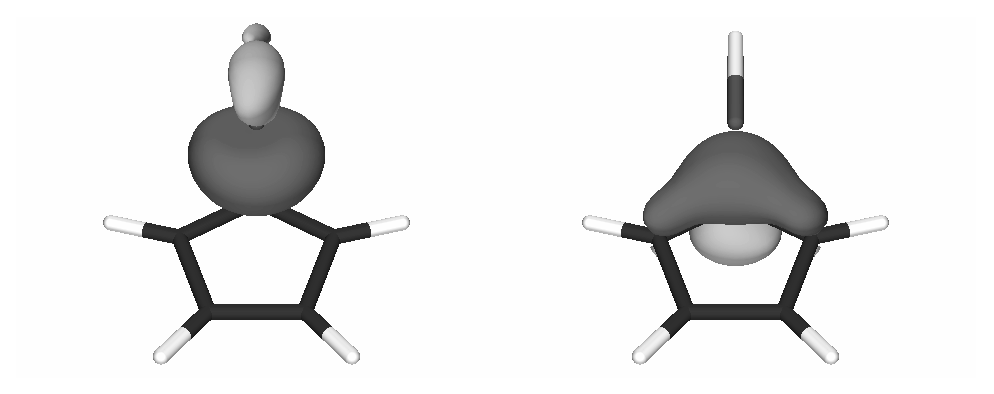
\includegraphics[scale=0.6]{orbopt/figures/sigma_sih.eps}
\caption{The $\sigma$ bound structure of Cp-SiH. Shown are the two singly occupied orbitals: the $sp$ hybridized orbital on SiH (left) and a $p$ orbital on the Cp-ring (right).}
\label{fig.cpsih}
\end{figure}
The calculation on this molecule forms a useful example for testing the additions to the optimization options, because the VBSCF process changes the orbitals drastically (in this case the total energy drops 0.86 Hartree between the initial and the final iteration). This is caused by the quality of the guess orbitals of which several are generated by hand instead of by a preceding Hartree-Fock calculation.

The molecule consists of two separate fragments, or \textit{hybrids} as they are referred to in TURTLE, \textit{i.e} the cyclopentadienyl part and the siliconhydride part. In these parts the doubly occupied orbitals are orthogonal to each other, to the variably occupied and virtual orbitals inside their \textit{hybrid}. However, the \textit{hybrids} are not necessarily orthogonal to one another. In this case the orbitals in the cyclopentadienyl \textit{hybrid} are not orthogonal to the orbitals in the siliconhydride \textit{hybrid} and therefore the \textit{fock} option cannot be used.

For the original calculations TURTLE's \textit{super} option, which ensures that only excitations to virtual (unoccupied) orbitals are included in Super CI, was used. Without the \textit{super} option excitations to partly occupied orbitals are included as well. The reason was that the excitations from occupied orbitals in one structure to a partly vacant orbital in the same or in an other structure resulted in convergence problems. For the specification of the \textit{pert} option via orbital classes, this means that only excitations from doubly to unoccupied orbitals \mbox{(doc-uoc)} and excitations from variably to unoccupied orbitals \mbox{(voc-uoc)} have to be tested, since excitations from doubly occupied to variably occupied \mbox{(doc-voc)} and from variably to variably occupied orbitals \mbox{(voc-voc)} are not used in this \textit{super} VBSCF calculation.

Besides the effect of the \textit{pert} option, the effect of the convergence helpers DIIS \cite{diis1,diis2} and level shifting \cite{level1,level2} was analyzed. In DIIS a successive set of iterations, of which each has an associated set of new orbitals and a gradient vector ($\mathbf{b}$), are used to guess the new orbitals. For more details and its use in TURTLE, see appendix III in \cite{koos1}. With the level shifter in TURTLE, the value of $\left < \Psi_0 | \mathbf{H} - E_0 | \Psi_0 \right >$ is lowered by a user specified amount during the diagonalization step. A useful value for the shifter, if any, is found by trial and error. DIIS, when applied, was used from the first iteration on. For the level shifter, when applied, only the value 1 was used. Furthermore, the convergence criterion was set to 1*10$^{-4}$ as maximum value for any of the Brillouin coefficients ($b_{ia}$, equation \ref{ch2.eq.superci}). This resulted in a total VB-energy which was, up to 5 decimal places, the same for all (converged) calculations: -481.44177 Hartree.

The results of the calculations are presented in Table \ref{ch2.tab.budzelaar}.
\begin{table}[htdp]
\caption{Timings in seconds of the VBSCF calculations on Cp-SiH (with the number of iterations between parenthesis). Three different optimization types were tested, regular Super CI, doc-uoc and doc-uoc/voc-uoc. With these different optimization types a combination of two convergence aids, DIIS and a level shifter (only for the \textit{pert} calculations) have been applied.}
\begin{center}
\begin{tabular}{l c c}
\hline
Type & no DIIS & DIIS \\
\hline
\textit{superci} & 3349 (11) & 2735 (9) \\ 
\textit{pert} doc-uoc & 1368 (99) & 324 (23)\\ 
\textit{pert} doc-uoc/voc-uoc & 1172 (98) & 316 (26)\\
\end{tabular}
\label{ch2.tab.budzelaar}
\end{center}
\end{table}
Without the convergence aid of a level shifter the calculations on this molecule with the \textit{pert} option switched on did not converge, while the regular Super CI calculation converged successfully in 11 iterations after 3349 seconds. Although the number of iterations needed to reach convergence is much larger than for a Super CI calculation, the total timings for the calculations with the \textit{pert} option are significantly lower. This is because the number of matrix elements necessary for \textit{pert} is much lower and therefore each iteration takes less time, but on the other hand information is discarded by leaving out matrix elements which results in (much) more iterations. 

Switching on DIIS appeared to be very beneficial for the \textit{pert} calculations, since it reduced the number of iterations roughly by a factor of four (Table \ref{ch2.tab.budzelaar}). For the \textit{superci} calculation DIIS was also advantageous: the calculation was shortened by almost 20\%.

\subsection{\label{ch2.sec.aromat}Second Example: Cyclic Hydrocarbons}

Aromaticity has been and still is widely studied using Valence Bond theory \cite{cooper1,cooper2,remcolowdin,indacene,fowler,jenneskens,cyclohexatriene,bestbenzene,benzyne}. The molecules involved are planar, having a strict separation of the $\sigma$ and $\pi$ system. For the test four planar molecules, cyclobutadiene (\textbf{1}), benzene (\textbf{2}), cyclooctatetraene (\textbf{3}) and pentalene (\textbf{4}) have been selected (Figure \ref{ch2.fig.compounds}).
\begin{figure}[htdp]
\center
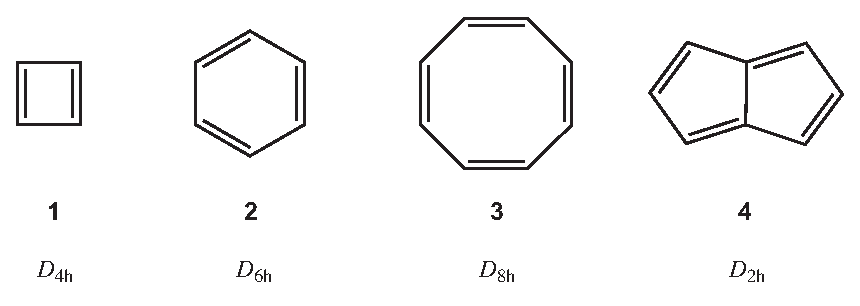
\includegraphics[scale=0.85]{orbopt/figures/compounds.eps}
\caption{Cyclobutadiene (\textbf{1}), benzene (\textbf{2}), cyclooctatetraene (\textbf{3}) and pentalene (\textbf{4}). Underneath the compound numbers the symmetry used for the respective compounds has been printed.}
\label{ch2.fig.compounds}
\end{figure}

Prior to any VB calculation, the geometry of the compounds had been optimized in the symmetry indicated in Figure \ref{ch2.fig.compounds}, using Restricted Hartree-Fock (RHF) with the \mbox{6-31G} basis set \cite{631g1,631g2}. The Valence Bond calculations, three per molecule, using the \textit{superci}, \textit{pert} and \textit{fock} options, were performed using delocalized $\sigma$ orbitals and strictly atomic $\pi$ orbitals, generated by a RHF calculation and an atomic SCF, respectively, all in the 6-31G basis. For all VB calculations, the DIIS option was switched on from the start. TURTLE's \textit{hybrid} option was used to separate the $\pi$ orbitals from each other and the $\sigma$ core. \textit{All} excitations were treated with perturbation, both for \textit{pert} and for \textit{fock}. In this case the \textit{fock} option can be used for the doubly occupied orbitals in the $\sigma$ core, because of the orthogonality of the $\pi$ orbitals to the $\sigma$ core. 

In Table \ref{ch2.tab.flat1} and \ref{ch2.tab.flat2} the results are presented. The total energies, presented below the name of each compound in the tables, was equal for all optimization methods for the first eight decimal places. Beneath the energies, for all methods the number of iterations, the total timings and the speed-up factors compared to regular Super CI are presented. In the case of the \textit{fock} option only the orbitals from the $\sigma$ core are optimized using the Fock algorithm; the $\pi$ orbitals are optimized using the \textit{pert} option in that case.

\begin{table}[htbp]
\caption{Below their names, the total energy of both molecules is presented. The number of iterations, timing per iteration and speed-up factors (compared to \textit{superci}) for butadiene and benzene.}
\begin{center}
\begin{tabular}{l c c c c c c}
\hline
&\multicolumn{3}{c}{\textbf{Butadiene}}&\multicolumn{3}{c}{\textbf{Benzene}}\\
&\multicolumn{3}{c}{(-153.59682368 au)}&\multicolumn{3}{c}{(-230.54408700 au)}\\
\textbf{Method}&\textbf{\# iter}&\textbf{sec/iter}&\textbf{speed-up}&\textbf{\# iter}&\textbf{sec/iter}&\textbf{speed-up}\\
\hline
\textit{superci}&8&73.0&1&8&2274.1&1\\
\textit{pert}&14&4.9&8&13&90.8&15\\
\textit{fock}&10&4.8&12&10&79.3&23\\
\end{tabular}
\label{ch2.tab.flat1}
\end{center}
\end{table}

\begin{table}[htbp]
\caption{Below their names, the total energy of both molecules is presented. The number of iterations, timing per iteration and speed-up factors (compared to \textit{superci}) for cyclooctatetraene and pentalene.}
\begin{center}
\begin{tabular}{l c c c c c c}
\hline
&\multicolumn{3}{c}{\textbf{Cyclooctatetraene}}&\multicolumn{3}{c}{\textbf{Pentalene}}\\
&\multicolumn{3}{c}{(-307.35606250 au)}&\multicolumn{3}{c}{(-306.14034868 au)}\\
\textbf{Method}&\textbf{\# iter}&\textbf{sec/iter}&\textbf{speed-up}&\textbf{\# iter}&\textbf{sec/iter}&\textbf{speed-up}\\
\hline
\textit{superci}&8&320106.0&1&8&47692.8&1\\
\textit{pert}&13&4704.2&42&14&1982.4&14\\
\textit{fock}&10&3857.0&66&12&1386.8&23\\
\end{tabular}
\label{ch2.tab.flat2}
\end{center}
\end{table}

For all molecules, the Super CI calculations take 8 iterations. Both in the \textit{fock} and in the \textit{pert} calculations more iterations are necessary to reach convergence. The approximation of the diagonal matrix element (Section \ref{ch2.sec.denominator}) seems to be beneficial for the calculation, because the number of iterations for \textit{fock} is smaller than for \textit{pert} in all four situations.

From the timings, it becomes clear that the \textit{fock} option is fruitful for this type of molecule, because the speed-up lies between 12 times for butadiene to 66 times for cyclooctatetraene compared to traditional Super CI. The difference between the speed-up of \textit{fock} and \textit{pert} is reasonable, but not as impressive as the difference between \textit{pert} and \textit{superci}. A drawback of the \textit{fock} option is the orthogonality condition that has to be met. 

Delocal VBSCF calculations, for which no examples have been presented here, do not suffer from this drawback, because in those calculations the doubly occupied orbitals will be orthogonal to each other, to the variably occupied orbitals and to the virtuals. However, most VB calculations in this thesis have been run with the \textit{hybrid} option, for which the \textit{fock} option is restricted to special cases, where the different \textit{hybrids} are orthogonal by symmetry.

% Not here, zegt Joop :
%The \textit{pert} option is more generally applicable, although in some cases, like in the first example, convergence aids are necessary to make the calculations converge, as seen before.

\section{Conclusions}

Fock matrix elements, which can be calculated faster than Brillouin matrix elements, can be used for all excitations for which the orbital from which the excitation takes place (usually the doubly occupieds) and the orbital to which the excitation is, are orthogonal to each other and to the other orbitals. The other orbitals are allowed to be non-orthogonal to one another. In combination with the \textit{hybrid} option the \textit{fock} option can only be used when the doubly occupied orbitals in different \textit{hybrids} are orthogonal to all other orbitals.

When Fock matrix elements can be used, the calculation takes less time with the \textit{fock} than with the \textit{pert} option. However, the difference between \textit{fock} and \textit{pert} is not as impressive as the difference between \textit{pert} or \textit{fock} and \textit{superci}. Furthermore, the \textit{fock} option is not as generally applicable as the \textit{pert} option, because the latter does not require any orthogonality amongst the orbitals.

\section{Outlook}

A drawback of the current implementation of the \textit{pert} and \textit{fock} options is that they are not automatic. A first extension would be the implementation of an automatic \textit{pert}/\textit{fock} option. For each excitation only the first column element and the diagonal element, \textit{e.g.} $\left < \Psi_{0} | \mathbf{H} - E_0 | \Psi_{ia} \right >$ and $\left < \Psi_{ia} | \mathbf{H} - E_0 | \Psi_{ia} \right >$, are calculated. With these two elements the orbital update coefficient $b_{ia}$ is calculated. Only when its absolute value is above a predefined threshold the other Brillouin matrix elements for the excitation are calculated. For small update coefficients the \textit{pert} (or \textit{fock} if the situation permits it) option is then automatically used, since no other Brillouin matrix elements are calculated. 

Another step towards an automatic \textit{pert}/\textit{fock} option would be the use of orbital energies. Orbitals, like core $\sigma$ orbitals have a low energy ($i$ in Figure \ref{ch2.fig.energy}). %
% Helaas een newpage, want anders komt plaatje tussen referenties.
% (toch weer niet)
%\clearpage
%\newpage
%
\begin{figure}[ht]
\center
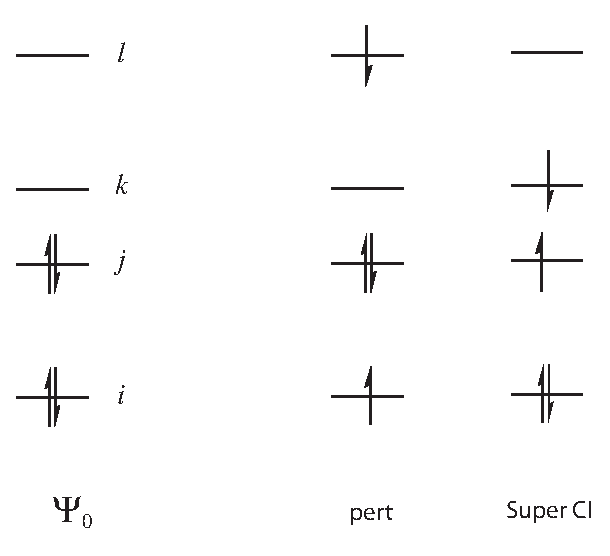
\includegraphics[width=2.8in]{orbopt/figures/orbitals.eps}
\caption{A wave function ($\Psi_0$), with two doubly occupied orbitals, one low lying ($i$) and one high lying ($j$). There are two virtual orbitals, one low lying ($k$) and one high lying ($l$). The excitation from $i$ to $l$ should be treated with the \textit{pert} option, while the excitation from $j$ to $k$ should be treated with regular Super CI.}
\label{ch2.fig.energy}
\end{figure} 
Excitations from these low lying orbitals to high lying virtuals ($l$) will only slightly change the wave function. Therefore, these orbitals  could easily be optimized by \textit{pert} or \textit{fock}. The HOMO-LUMO range ($j$, $k$), can be optimized by Super CI, since these orbitals are expected to change more than core orbitals. For the orbital energies the eigenvalues of a one electron operator on MO basis could be used.  Although these values are  estimates (interaction between orbitals is not taken into account), they can probably be used to separate between the excitations to be treated with the \textit{superci} and the \textit{pert} or \textit{fock} option. 

The use of the \textit{fock} option in combination with the \textit{hybrid} option may be used at this moment. However, it is assumed that the user will only use this combination when the doubly occupied orbitals in different \textit{hybrids} are orthogonal. An automatic orthogonality check for doubly occupied orbitals from different \textit{hybrids} would be desirable. In case of non-orthogonality, TURTLE should automatically use \textit{pert} instead of \textit{fock}. 

\section*{Appendix A: Cofactors}

A cofactor is a signed minor \cite{aitken}. A minor is created by removing one or more rows and columns from a determinant. Minors have the same sign as the original determinant from which they are derived. For a cofactor the sign depends on the position of the deleted row and column \cite{fokkeproef}. In this chapter the orbital overlap determinant, from which no rows and columns are removed, will be referred to as zeroth order cofactor. For a first order cofactor, obtained by removing one row and one column from the original determinant, the sign is $-1^{x+y}$, in which $x$ and $y$ are the indices of the deleted row and column. For a second order cofactor, obtained by removing two rows and two columns from the original determinant, the sign is $-1^{x_1+x_2+y_1+y_2}$, in which $x_1$, $x_2$, $y_1$ and $y_2$ are the indices of the deleted rows and columns. 

The overlap between two determinants can be expressed as  a zeroth order cofactor. The overlap of $\Delta_{1} = |ijkl \cdots n|$ with $\Delta_{2} = |ajkl \cdots n|$ for normalized orbitals is, \textit{e.g.}:
\begin{equation}
S_{12}^{(0)}=
\begin{array}{lllllll}
 &  i & j & k & l & \cdots & n \\
 a &  \multicolumn{1}{|l}{s_{ia}} & s_{ja}  & s_{ka} & s_{la} & & \multicolumn{1}{l|}{ s_{na} } \\
 j & \multicolumn{1}{|l}{s_{ij}} & 1 & s_{kj} & s_{lj} & & \multicolumn{1}{l|}{s_{nj}} \\
 k & \multicolumn{1}{|l}{s_{ik}} & s_{jk} & 1 & s_{lk} & & \multicolumn{1}{l|}{s_{nk}} \\
 l & \multicolumn{1}{|l}{s_{il}} & s_{jl} & s_{kl} & 1 & & \multicolumn{1}{l|}{s_{nl}} \\
 \vdots & \multicolumn{1}{|l}{ } &   &   & & \ddots & \multicolumn{1}{l|}{\vdots} \\
 n & \multicolumn{1}{|l}{ s_{in}} & s_{jn} & s_{kn} & s_{ln} & \cdots & \multicolumn{1}{l|}{1}
\end{array},\\
\label{ch2.eq.zocofac}
\end{equation}
in which the $s_{xy}$ elements stand for the orbital overlaps, \textit{i.e.} $\left < x | y \right >$. Along the rows and columns orbital labels are shown for readability. In the notation $S_{12}^{(0)}$, the superscript $(0)$ indicates that this is a zeroth order cofactor. The subscript $12$ indicates that the cofactor is constructed from overlaps of orbitals in determinant $\Delta_1$ with those from determinant $\Delta_2$.

A first order cofactor is derived from the zeroth order cofactor by removing one row and one column. So, when the column labeled $i$ and the row labeled $a$ are removed, the first order cofactor $S_{12}^{(i,a)}$ emerges:
\begin{equation}
S_{12}^{(i,a)} =
\begin{array}{lllllll}
 &  \hskip 2.0 pt \hbox{\lower 120pt\hbox{\vrule height128pt width 1.0pt}}\hskip-3.0pt i & j & k & l & \cdots & n \\
\noalign{\vskip-115pt}
 a &  \multicolumn{1}{|l}{s_{ia}} & s_{ja}  & s_{ka} & s_{la} & & \multicolumn{1}{l|}{ s_{na} } \\
\noalign{\vskip-8pt}
\multispan7\hbox{\vrule  height 1.0 pt width164pt}\cr
\noalign{\vskip 7pt}
  j & \multicolumn{1}{|l}{s_{ij}} & 1 & s_{kj} & s_{lj} & & \multicolumn{1}{l|}{s_{nj}} \\
 k & \multicolumn{1}{|l}{s_{ik}} & s_{jk} & 1 & s_{lk} & & \multicolumn{1}{l|}{s_{nk}} \\
 l & \multicolumn{1}{|l}{s_{il}} & s_{jl} & s_{kl} & 1 & & \multicolumn{1}{l|}{s_{nl}} \\
 \vdots & \multicolumn{1}{|l}{ } &   &   & & \ddots & \multicolumn{1}{l|}{\vdots} \\
 n & \multicolumn{1}{|l}{ s_{in}} & s_{jn} & s_{kn} & s_{ln} & \cdots & \multicolumn{1}{l|}{1}
\end{array}.\\
\label{ch2.eq.focofac}
\end{equation}
Since orbital $i$ is in the first column and orbital $a$ on the first row, the sign of the cofactor does not change because $-1^{(1+1)} = +1$.

When the columns labeled $i$ and $k$ and the rows labeled $a$ and $l$ are removed from $S_{12}^{(0)}$ the second order cofactor $S_{12}^{(i,k,a,l)}$ is generated:
\begin{equation}
S_{12}^{(i,k,a,l)} =
\begin{array}{lllllll}
 &  \hskip 2.0 pt \hbox{\lower 120pt\hbox{\vrule height128pt width 1.0pt}}\hskip-3.0pt i & j & \hskip 2.0 pt \hbox{\lower 120pt\hbox{\vrule height128pt width 1.0pt}}\hskip-3.0pt k & l & \cdots & n \\
\noalign{\vskip-115pt}
 a &  \multicolumn{1}{|l}{s_{ia}} & s_{ja}  & s_{ka} & s_{la} & & \multicolumn{1}{l|}{ s_{na} } \\
 \noalign{\vskip-8pt}
\multispan7\hbox{\vrule  height 1.0 pt width164pt}\cr
\noalign{\vskip 7pt}
 j & \multicolumn{1}{|l}{s_{ij}} & 1 & s_{kj} & s_{lj} & & \multicolumn{1}{l|}{s_{nj}} \\
 k & \multicolumn{1}{|l}{s_{ik}} & s_{jk} & 1 & s_{lk} & & \multicolumn{1}{l|}{s_{nk}} \\
 l & \multicolumn{1}{|l}{s_{il}} & s_{jl} & s_{kl} & 1 & & \multicolumn{1}{l|}{s_{nl}} \\
 \noalign{\vskip-8pt}
\multispan7\hbox{\vrule  height 1.0 pt width164pt}\cr
\noalign{\vskip 7pt}
 \vdots & \multicolumn{1}{|l}{ } &   &   & & \ddots & \multicolumn{1}{l|}{\vdots} \\
 n & \multicolumn{1}{|l}{ s_{in}} & s_{jn} & s_{kn} & s_{ln} & \cdots & \multicolumn{1}{l|}{1}
\end{array}.\\
\label{ch2.eq.socofac}
\end{equation}
In this second order cofactor the sign changes, because the position of the orbitals is: $i$ in the first and $k$ in the third column, $a$ on the first and $l$ on the fourth row. This makes $-1^{(1+3+1+4)} = -1$.

\bibliography{orbopt}
\bibliographystyle{../main/achemso}
